
\subsection{Clustering}

We manually inspect our clusters for both high similary of articles within clusters and ow similarity of articles between clusters. Since we do not have a gold standard for news event labels, we cannot calculate values such as true positives and true negatives. We present some qualitative results.

\textbf{First ten articles of Cluster 0:}  
\begin{enumerate}
\item Retrial of 3 Al-Jazeera journalists (Egypt)
\item Protests for seizing of hospital accounts (DR Congo)
\item Waterloo homicide arrest (England)
\item Taliban vs Afghan army (Afghanistan)
\item \$20 million funding for Wilmington pharmacy (Delaware)
\item Tiger farms violate Endangered Species Law (China)
\item DeSoto corruption trial (Mississippi)
\item Six die at David Owuor's Nakuru crusade (Kenya)
\item Temp workers fight for wages (Chicago)
\item Grant of bail to Lakhvi, mastermind of Mumbai attack (Pakistan)
\end{enumerate}

As can be seen, purity for cluster 0 is fairly high, with seven of ten articles dealing with judicial decisions. In general, most clusters appear to have reasonable purity, but there is also high similarity between clusters. For example, articles similar to the first article in cluster 0 also appear in cluster 5. Cluster 5 is similar to cluster 0 in that they both deal with judicial decisions.\\

\noindent A search for the name of the mastermind of the Mumbai attacks, Zakiur Rehman Lakhvi, returned results in 69 of 1000 clusters, which indicates we have much more cross-cluster similarity than we'd like. But this is a more preferable problem to have than a lack of intra-cluster similarity. Our eyeball test can only evaluate cluster quality based on keywords such as actor names and locations and general topics. Its possible that Lakhvi can appear in 69 clusters because the other metrics articles are clustered on, such as tone or the importance features, which an eyeball test cannot detect, do in fact separate Lakhvi related articles into that many clusters.

\subsection{Regression}
\begin{figure}[H]
	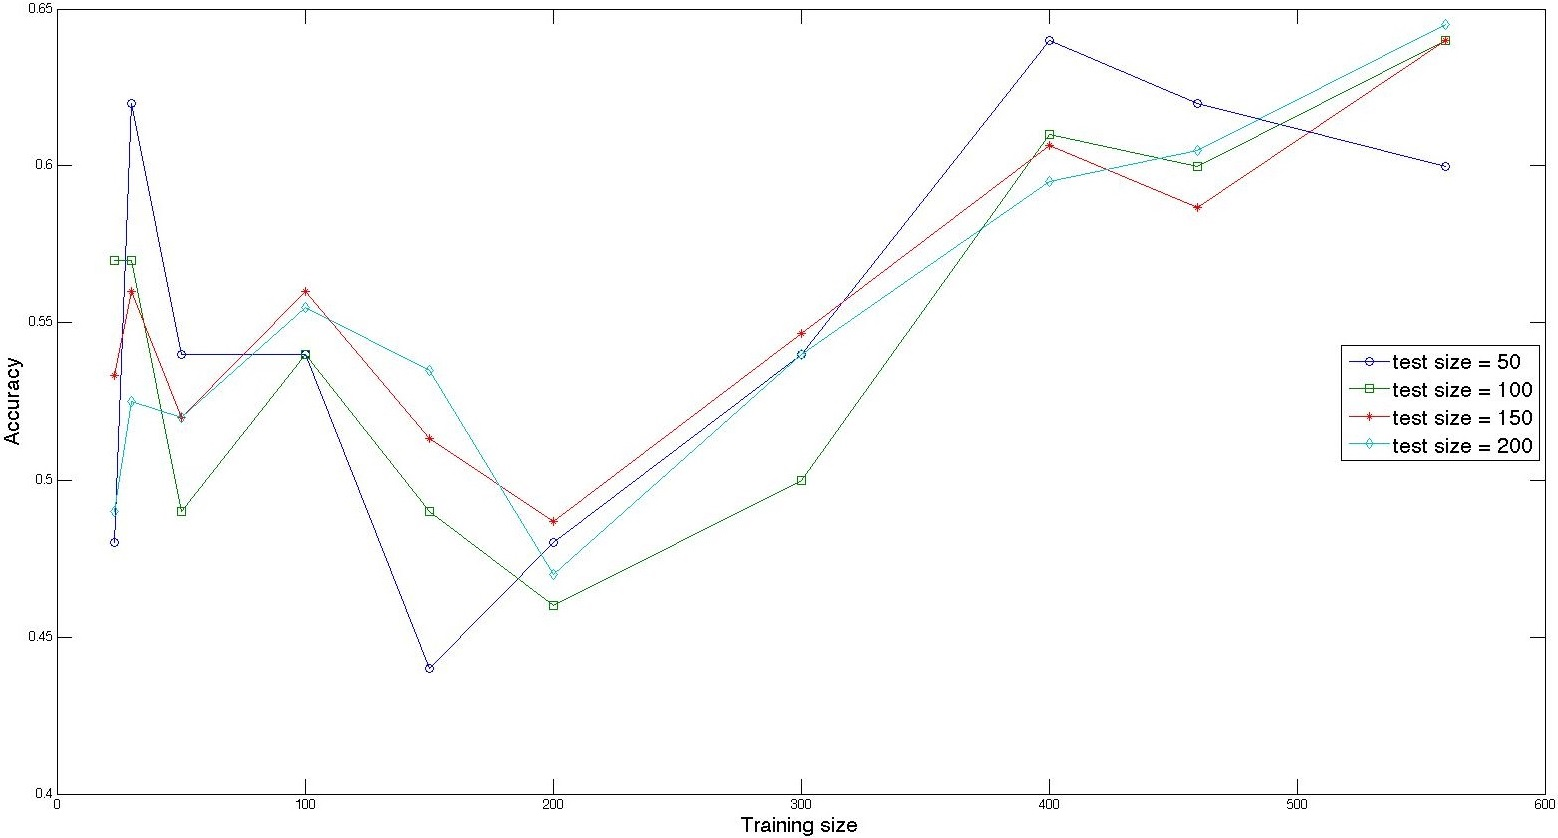
\includegraphics[width=0.5\textwidth]{results/acc.jpg}
	\caption{Accuracy for various test sizes}
\end{figure}
\begin{figure}[H]
	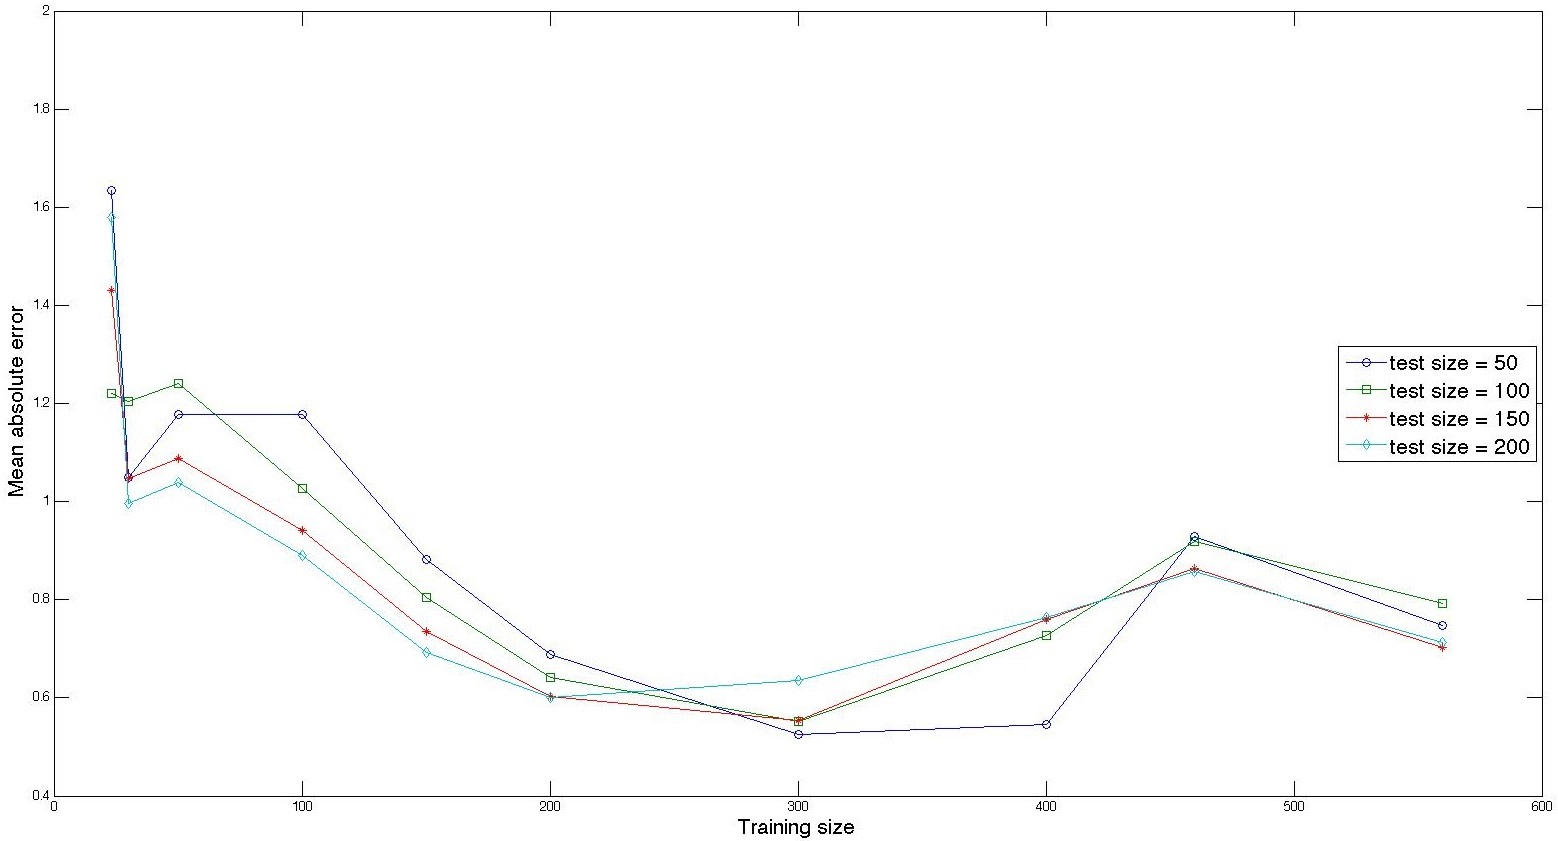
\includegraphics[width=0.5\textwidth]{results/mae.jpg}
	\caption{Mean aboslute error for various test sizes}
\end{figure}
\figurename{6} and \figurename{7} show the accuracy and mean absolute error across test size for a fixed window of last 22-560 training days.
\begin{figure}[H]
	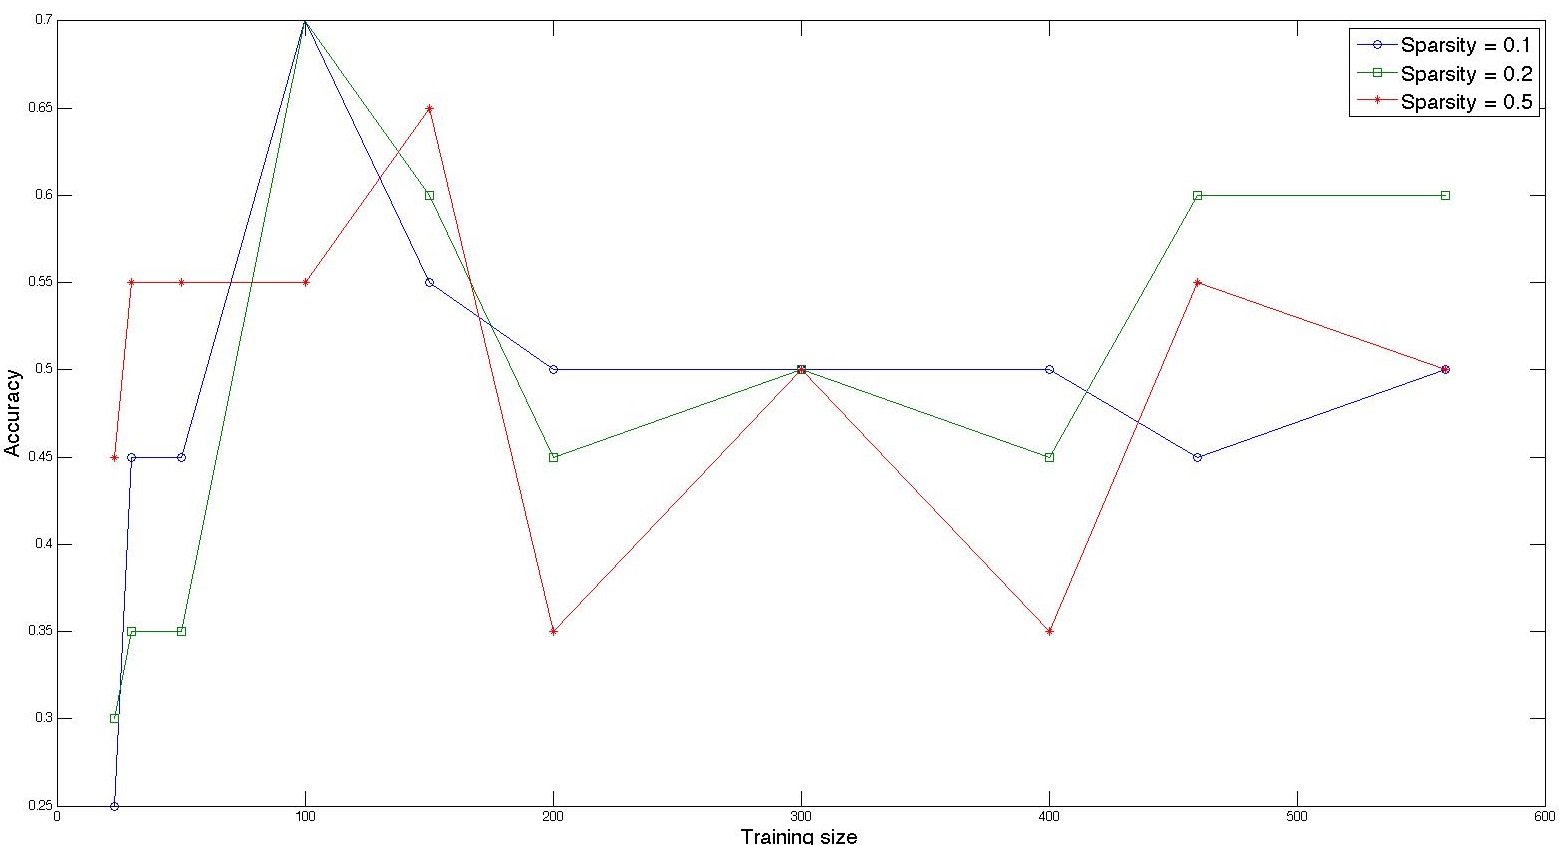
\includegraphics[width=0.5\textwidth]{results/acc2.jpg}
	\caption{Accuracy for various sparsity}
\end{figure}
\begin{figure}[H]
	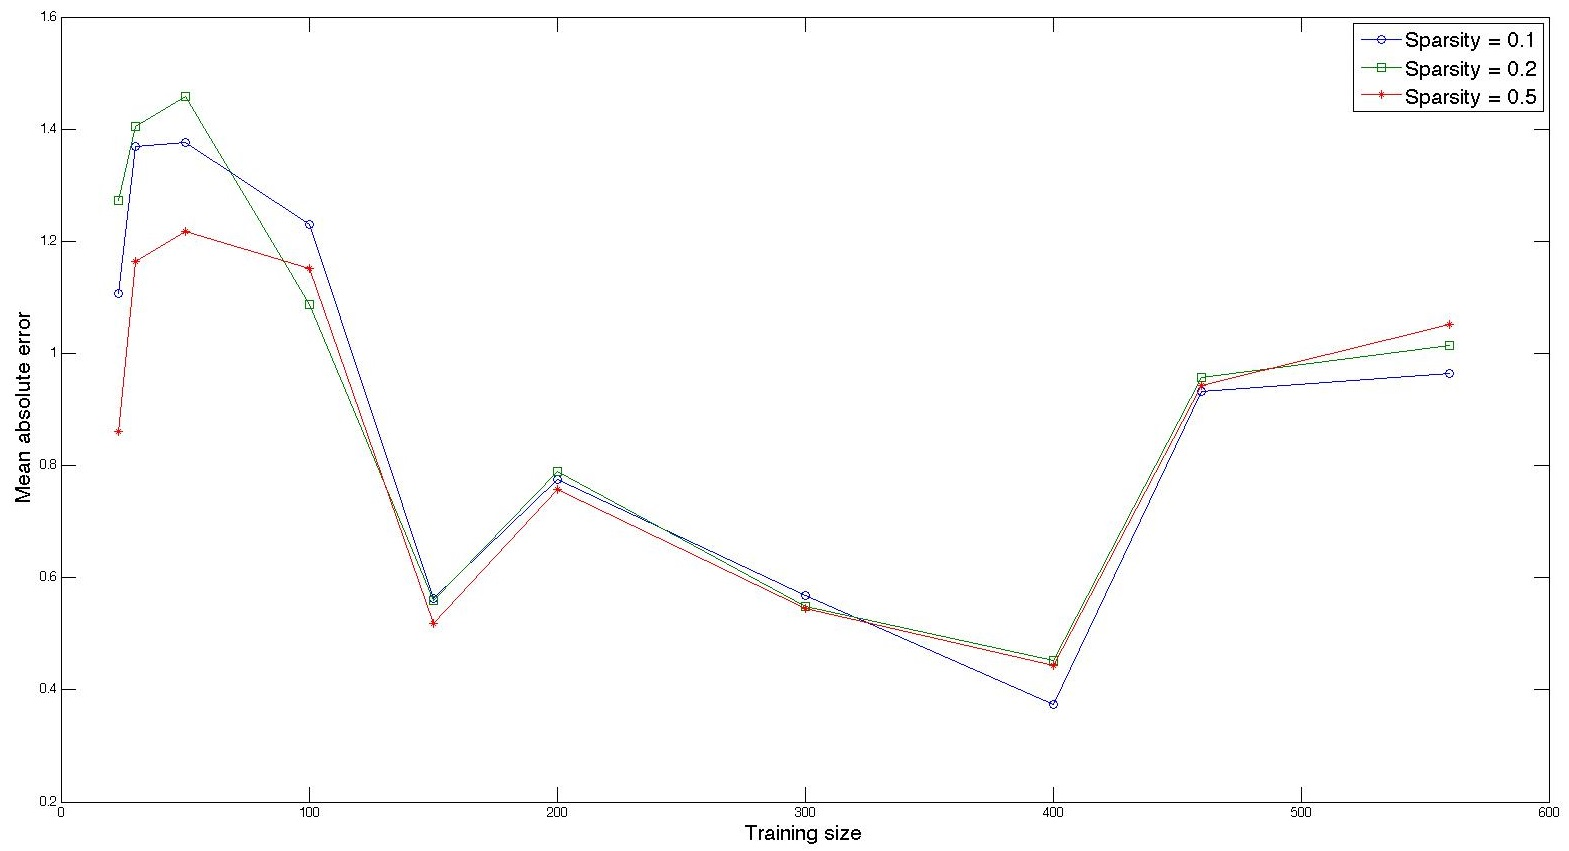
\includegraphics[width=0.5\textwidth]{results/mae2.jpg}
	\caption{Mean abolsute error for various sparsity}
\end{figure}

\figurename{8} and \figurename{9} show the accuracy and mean absolute error across sparsity for a moving window of last 22-560 training days

\begin{figure}[h!]
	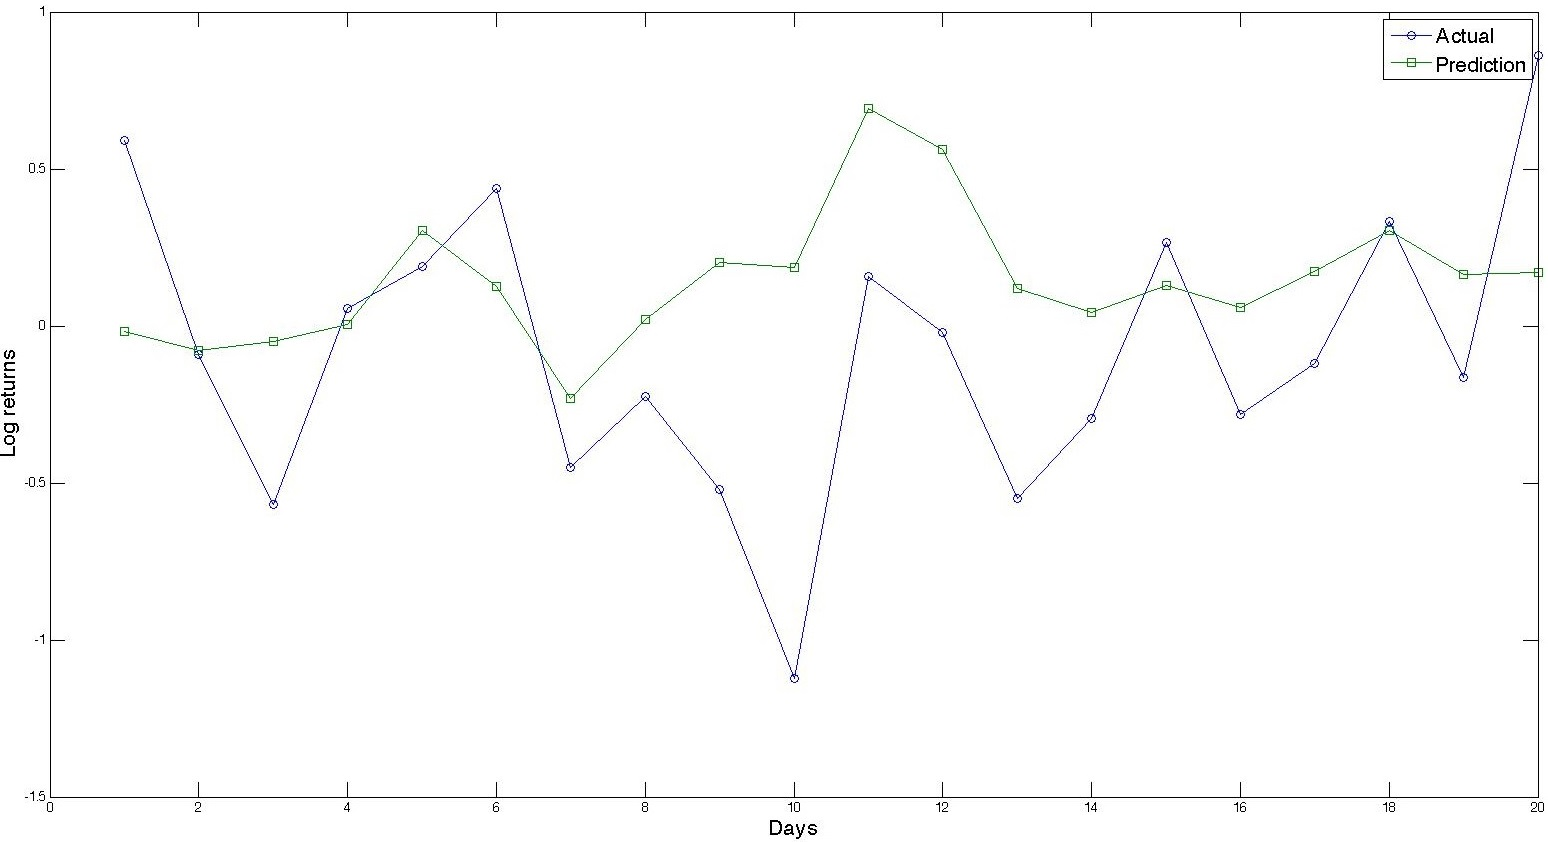
\includegraphics[width=0.5\textwidth]{results/prediction.jpg}
	\caption{Comparison of log returns for sparsity = 0.1, training size = 400}
\end{figure}

\figurename{10} is a log return plot with a moving window of 400 days and sparsity 0.1 having a mean absolute error of 0.37.



